% !TEX root = monografia.tex
\chapter{Solucionando o problema}
\label{cap:solucao}

Atacaremos o problema com a seguinte abordagem, chamada de \textit{gradiente de política}: vamos definir uma \textit{parametrização} da política, ou seja, uma família de funções da forma $\pi_{\theta}(a | s) = \mathbb{P}(A_t = a | S_t = s, \theta_t = \theta)$ e uma função objetivo $\mathcal{J}(\theta)$ de tal forma que nosso problema se reduz a encontrar um vetor $\theta \in \mathbb{R}^d$ que maximiza a função $\mathcal{J}$. Para isso, utilizaremos o gradiente da função $\mathcal{J}$, por isso temos que escolher $\pi$ e $\mathcal{J}$ diferenciáveis em $\theta$.

Vale notar que essa abordagem é até aqui idêntica a abordagem padrão utilizada em problemas de Aprendizado Supervisionado Profundo. A diferença estará na definição da função $\mathcal{J}$ e, por consequência, como iremos calcular seu gradiente. Podemos fazer a distinção entre 2 elementos do algoritmo: o \textit{modelo} (que corresponde a escolha da parametrização da política) e o \textit{método de otimização} (que é o algoritmo que encontrará um vetor de parâmetros satisfatório).

\section{Modelo}

O nosso modelo será um Rede Neural Convolucional (?). Com um poder de representatividade muito grande e acompanhadas de poderosos métodos de otimização, modelos baseados em Redes Neurais têm batido recordes em um grande número de tarefas em Aprendizado de Máquina (?).

\subsection{Redes Neurais}

\begin{figure}[h!]
\centering
    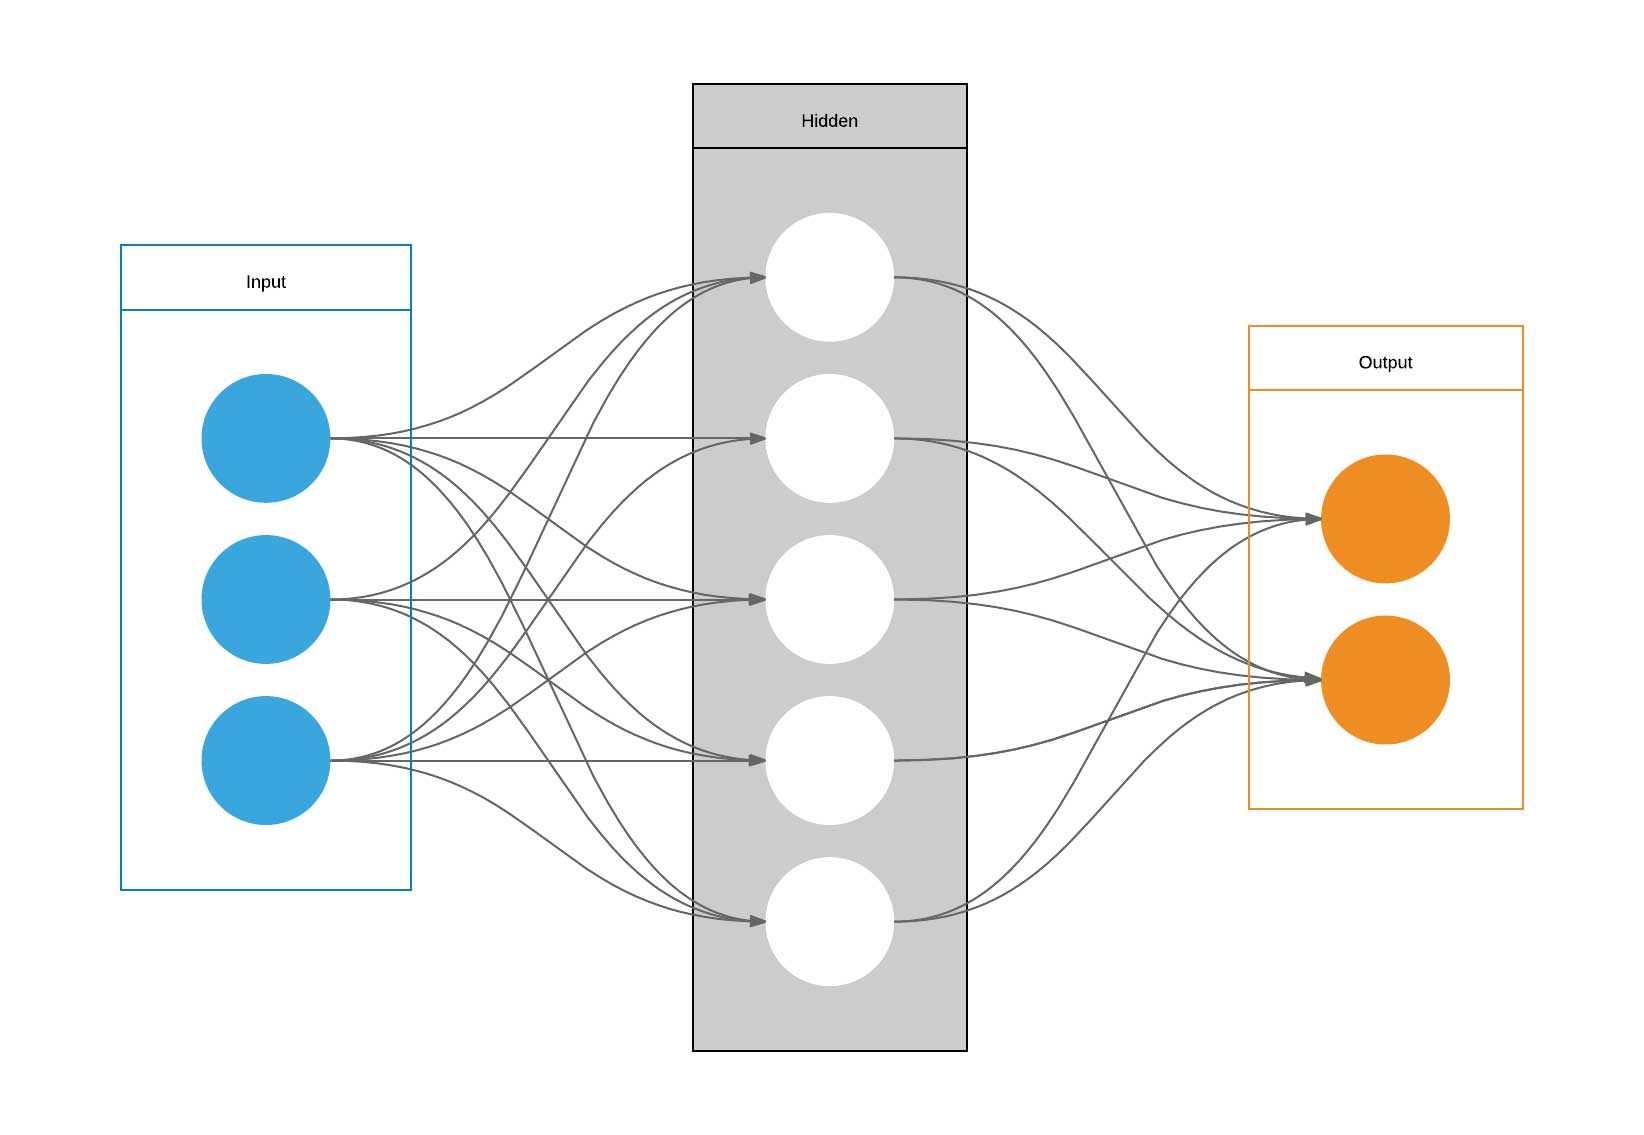
\includegraphics[width=8cm]{figuras/nn}
    \caption{Uma Rede Neural simples}
    \label{fig:nn}
\end{figure}

Uma Rede Neural é essencialmente uma composição de várias funções simples, chamadas de \textit{neurônios}. Um neurônio é em geral uma função da forma $\sigma(T(x; \theta))$, onde $T$ é uma função linear e $\sigma$ é uma função não linear (diferenciável).

Redes Neurais possuem um poderoso algoritmo chamado de \textit{retroprogagação} (em inglês \textit{backpropagation}) (?) para calcular a derivada do modelo inteiro de uma forma eficiente.

As Redes Neurais Convolucionais são Redes Neurais que explicitamente colocam no modelo hipóteses sobre a distribuição espacial dos dados, principalmente através de assumir que a informação está codificada em uma matriz quadrada (ou várias delas) de forma invariante a translação. Esse tipo de rede têm sido revolucionária na área de visão computacional (?), e é próprio a aplicação delas aqui, já que o estado do jogo é comunicado através de um mapa quadricular que respeita essas hipóteses. Falaremos mais sobre elas no capítulo sobre nosso modelo.

\begin{figure}[h!]
\centering
    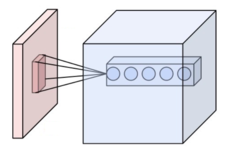
\includegraphics[width=8cm]{figuras/Conv_layer.png}
    \caption{Uma Rede Neural Convolucional}
    \label{fig:conv_layer}
\end{figure}

\subsection{Hiperparâmetros}

É comum em Aprendizado de Máquina em geral e Aprendizagem Profunda em específico a presença de várias variáveis que não são otimizadas pelo algoritmo de otimização utilizado (em Aprendizagem Profunda elas surgem quando a função objetivo não é diferenciável em função da variável). Estas variáveis são chamadas de \textit{hiperparâmetros}. De maneira geral, escolhemos hiperparâmetros de acordo com o melhor consenso da literatura atual e/ou uma busca exaustiva em várias opções.

\section{Método de Otimização}

O nosso algoritmo de otimização será uma variação de \textit{subida de gradiente} (?). Esse algoritmo,
que é a base dos algoritmos de otimização utilizados em Aprendizagem Profunda, consiste em fazer pequenos ajustes no parâmetro $\theta$ na direção do gradiente $\nabla \mathcal{J}(\theta)$, resumidamente, $\theta_{t + 1} = \theta_t + \gamma \nabla \mathcal{J}(\theta)$. A ideia do algoritmo vem do fato que, para um $\gamma$ suficientemente pequeno, teremos que $\mathcal{J}(\theta_{t+1}) > \mathcal{J}(\theta_{t})$ se o gradiente for diferente de 0.

\subsection{Função Objetivo}

Nossa função objetivo será escolhida como $\mathcal{J}(\theta) \doteq v_{\pi_{\theta}}(S_0)$, ou seja, o valor do estado inicial na política definida por $\theta$. Assim, diretamente adaptamos o objetivo dos nossos agentes como uma função de $\theta$.

Essa função é diferenciável e além disso temos uma forma conveniente de expressar seu gradiente através do teorema do gradiente de política (?):

\begin{equation}
    \nabla \mathcal{J}(\theta) 
    \propto \mathbb{E}_{\pi} \Big[ q_{\pi}(S_t, A_t) \frac{\nabla_{\theta} \pi_{\theta}(A_t | S_t)}{\pi_{\theta}(A_t | S_t)} \Big]
    = \mathbb{E}_{\pi} \Big[ G_t \frac{\nabla_{\theta} \pi_{\theta}(A_t | S_t)}{\pi_{\theta}(A_t | S_t)} \Big]
\end{equation}

Ou seja, podemos simular o ambiente, calcular a expressão entre os colchetes, e com ela fazer múltiplas atualizações do nosso parâmetro, obtendo uma aproximação estatística da subida de gradiente. Falta somente escolher o coeficiente de proporcionalidade, o $\gamma$ da subida de gradiente. Falaremos sobre essa escolha no capítulo sobre o método de otimização.

